\section{Prompts}
\label{app:prompts}
The instructions of the DSPy signatures used for the evaluation runs, verbatim. Input and output fields are omitted.

\begin{lstlisting}[title={LayerChildGenerationSignature (Phase 1, one layer of children)}]
Generate children for a specific parent node in the research DAG.
You are a research planning expert. Given a parent research question and the current DAG structure, generate focused sub-questions that can be answered independently to collectively answer the parent question. Look at the entire DAG context to ensure coherence and avoid duplication.
Guidelines:
1. Generate focused, standalone sub-questions that collectively answer the parent
2. Consider the existing DAG structure to maintain coherence
3. Respect the max_children limit strictly
4. Each child should be answerable independently
5. Output format should always be "list" (bullet points)
\end{lstlisting}

\begin{lstlisting}[title={CompositionInstructionSignature (Phase 1, per parent)}]
Write explicit parent composition instructions referencing each child node.
Given a parent node and its children, explain exactly how the child answers will be combined to produce the parent's output. Always reference children by their IDs so downstream steps can trace dependencies unambiguously.
\end{lstlisting}

\begin{lstlisting}[title={LeafNodeResearcher (Phase 2, leaves)}]
Answer a leaf node research task using literature search results.
Given literature search results and the expected output format, provide an answer that strictly adheres to the format requirements.
Format types and requirements:
- boolean: Provide "Yes." or "No." followed by a single sentence justification with citations.
- short_answer/list/report: Provide 3-5 bullet points ('- ' prefix) summarizing key takeaways with citations.
- table_csv/json: Provide structured data (CSV or JSON) with inline citations in headers or cells.
CRITICAL: Preserve all citations from the literature search in [X] format. Do not add citations that aren't in the source material.
\end{lstlisting}

\begin{lstlisting}[title={ParentNodeSynthesizer (Phase 2, parents)}]
Synthesize answers from child nodes to answer a parent node's research task.
Given the answers from all child subtasks and composition instructions, combine them to produce the answer for the parent task in the required format.
CRITICAL RULES:
1. Use ONLY the information from the child results - no external knowledge
2. Follow the composition instructions exactly
3. When citing evidence, use the citation numbers [1], [2], etc. from the AVAILABLE CITATIONS section - do NOT reference child nodes by name
4. Output in the specified format
5. If child results contradict, acknowledge and explain the contradiction
\end{lstlisting}

\begin{lstlisting}[title={GapExplorer (Phase 2, refinement, first pass)}]
Explore potential gaps that could enhance the composed answer.
This is the FIRST PASS - be creative and identify any areas where the answer could be improved, even if they're minor enhancements. Don't filter yet.
Think about: missing perspectives or viewpoints; unaddressed sub-questions or aspects; areas that could use more depth or detail; counterarguments or alternative viewpoints not covered; quantitative data or evidence gaps; temporal or geographic coverage gaps; edge cases or exceptions not mentioned.
Return a list of potential gaps, even if they seem minor. The second pass will determine which ones are critical enough to warrant refinement.
\end{lstlisting}

\begin{lstlisting}[title={GapImportanceEvaluator (Phase 2, refinement, second pass)}]
Evaluate whether identified gaps are important enough to warrant refinement.
This is the SECOND PASS - evaluate gaps based on the specified conservatism level.
CONSERVATISM MODES:
- "conservative": Only flag gaps that are CRITICAL - the answer would be misleading or fundamentally incomplete without this information. Default to NOT refining.
- "balanced": Flag gaps that would SIGNIFICANTLY improve the answer's completeness, depth, or accuracy. Be moderate - refine if the gap meaningfully enhances quality.
- "aggressive": Flag gaps that would improve the answer, even if moderately. Refine if the gap would add value, even if not critical.
Consider: Would adding this information fundamentally change the answer's conclusion? Is this gap misleading or would it cause the answer to be wrong? Would a reasonable reader say the answer is incomplete without this? Is this a core aspect of the question that's missing? How much would this gap improve the answer's quality?
Provide a confidence score (0.0-1.0) indicating how confident you are that refinement is warranted.
\end{lstlisting}

\begin{lstlisting}[title={OutlineFromDAGSignature (Phase 3)}]
Generate a report outline that structures a persuasive argument from DAG research.
The DAG represents a research question decomposed into sub-questions. Each node answered a question through research. The root node has the final answer; child nodes contain supporting evidence that led to that answer.
Create an outline for a persuasive report arguing a definitive stance for the root answer. Use the DAG's hierarchy to organize evidence: child findings support parent conclusions. Structure as a logical argument (Executive Summary, Evidence Sections, Conclusion).
REQUIREMENTS: Start with Executive Summary stating root answer prominently; organize body sections to build argument logically using DAG hierarchy; use ## for main sections, ### for subsections; design for prose writing (paragraphs, not just lists); base outline ONLY on content actually present in root_answer (no placeholders).
\end{lstlisting}

\begin{lstlisting}[title={ReportFromDAGSignature (Phase 3)}]
Generate a comprehensive final report from the DAG results.
The report must: 1. Start with the root answer prominently (matching its format) 2. Follow the provided outline structure 3. Incorporate findings from all DAG nodes 4. Take a clear stance that matches the root answer 5. Preserve all citations [X] from the DAG 6. Be well-written, coherent, and comprehensive
CRITICAL STANCE ALIGNMENT: If root answer is "Yes" (boolean), the report must argue FOR that position. If root answer is "No" (boolean), the report must argue AGAINST. If root answer is a list, the report should be organized around those items. The report's conclusion must align with the root answer. Do not contradict or hedge against the root answer's stance.
FORMATTING REQUIREMENTS: The report title (# heading) should be the CLAIM, not the question. Use proper markdown; write in prose paragraphs with supporting bullet points where appropriate; do not include internal node references in the output; only use citation numbers like [1], [2], [3]; every section must contain substantive content from the dag_results; do not include a bibliography section (it is added later).
\end{lstlisting}

\section{An Example DAG}
\label{app:dag}
\Cref{fig:dag} shows the DAG from a logged run on the motion ``Should the United States federal government substantially increase social services for persons living in poverty?'' with depth capped at 2. The planner split the root into the current landscape of services and the likely effects of expanding them, and each of those into two leaves. After composing the landscape node, the refinement check judged that child care and family tax credits were missing, and the pipeline attached a refinement sub-tree with two new leaves (shaded). The run's \dagLeaves{} leaves retrieved \dagLeafSources{} distinct sources, \dagLeafSourcesMean{} per leaf, and \dagRootFromRefinement{} of the root's \dagRootSources{} sources came from the refinement sub-tree, so refinement added about a third of the evidence. The final report has \dagReportWords{} words and \dagReportCitations{} citations and cites all \dagReportSources{} sources; \Cref{sec:citations} shows that its citations nonetheless do not match their claims. The full log, with every node's answer and citations, is in the repository.

\begin{figure}[t]
\centering
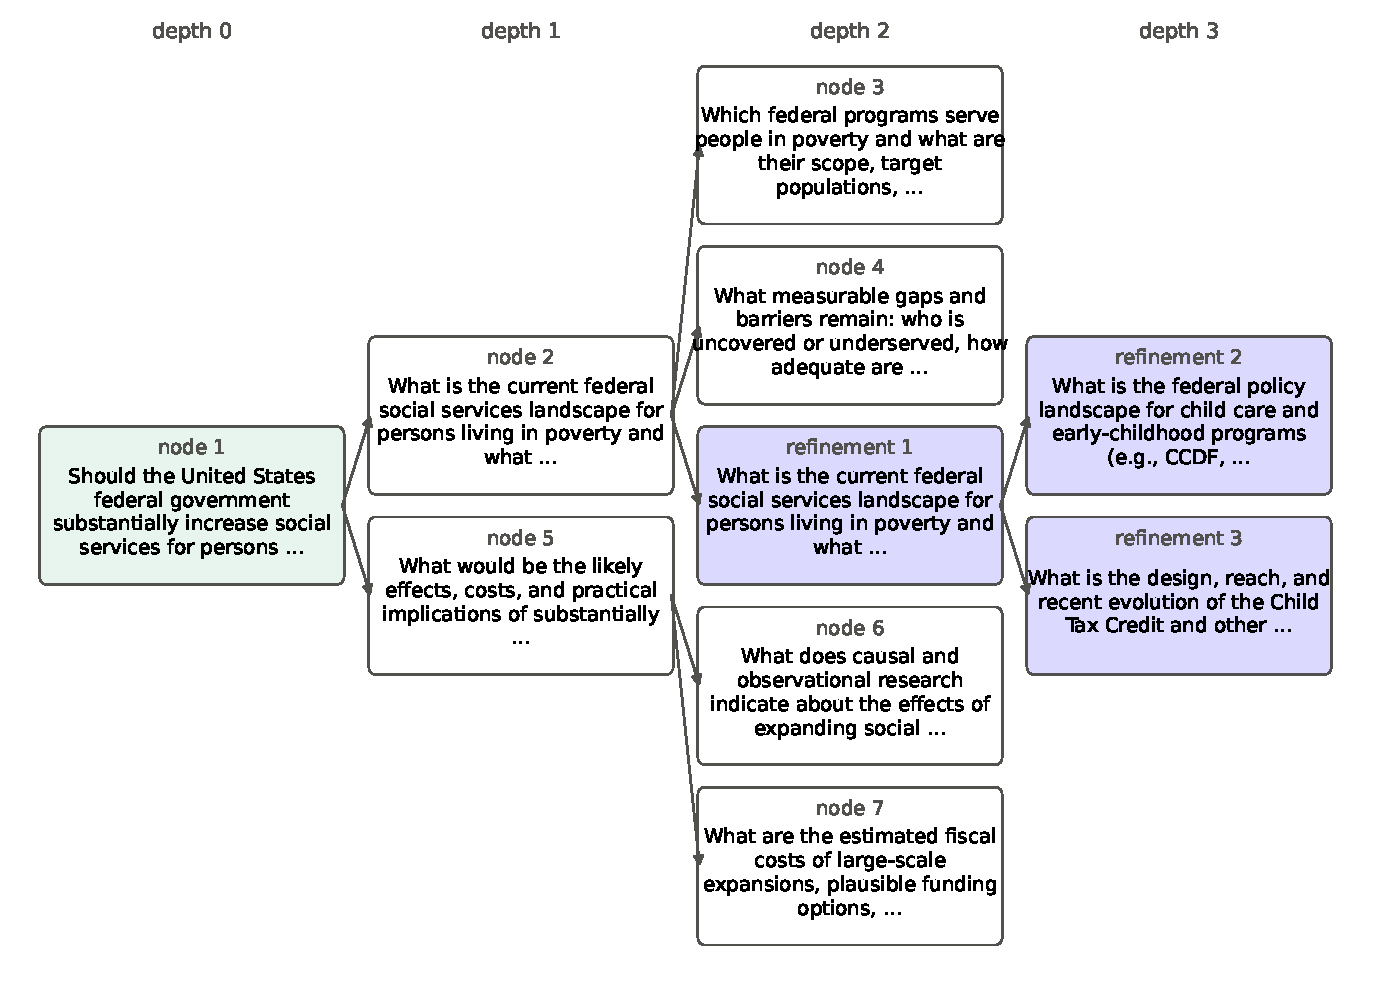
\includegraphics[width=\linewidth]{figs/example_dag.pdf}
\caption{A generated and refined DAG. Arrows point from parent to child. Shaded nodes were added by refinement after the composed answer of node 2 was judged incomplete.}
\label{fig:dag}
\end{figure}

\section{Code Versions}
\label{app:changes}
Three versions of the pipeline are involved, and only two are available.
\begin{enumerate}
    \item \textbf{Evaluated version.} The reports in \Cref{sec:experiments,sec:analysis} were finalized on 2 December 2025. Its prompts are the ones in \Cref{app:prompts}, taken from the authors' course write-up: the DAG is generated one layer at a time, composition instructions are written in a second pass, gaps are found by a two-pass explorer and evaluator, and the bibliography separates cited from uncited sources. This version's code is not in the public repository.
    \item \textbf{Repository version.} The last commit in the repository, from 26 November 2025, generates the whole DAG and its composition instructions in one call (\texttt{FullDAGGenerationSignature}) and checks gaps with one validator (\texttt{CompositionValidator}) that returns none unless a core aspect is missing. The logged run in \Cref{app:dag} comes from this version. Its citation handling is the one analyzed in \Cref{sec:mechanism}. The course write-up reports that citations were later given global numbers; that change is not in this version.
    \item \textbf{Released version.} The repository version with the provider made configurable, legacy code removed, and the citation fix of \Cref{sec:citations}: global citation numbers, node-reference expansion, the updated prompts, and the attribution audit (\texttt{utils/citations.py}, \texttt{utils/attribution\_audit.py}), with tests that replay the logged run.
\end{enumerate}
% CHECK with Justin: is the evaluated version (Gradescope submission) available? If so, add it to the repository and confirm whether its parent composition still passed leaf-local citation numbers.

\section{Report Statistics by Motion}
\label{app:reports}
\Cref{tab:reports} gives the length and sourcing of each retained report. The medians in \Cref{tab:text} are computed from these values.

\begin{table}[t]
\centering
\small
\begin{tabular}{p{6.4cm}rrrrr}
\toprule
Motion & \multicolumn{3}{c}{\sys{}} & \multicolumn{2}{c}{STORM} \\
\cmidrule(lr){2-4}\cmidrule(lr){5-6}
 & words & cited & listed & words & cited \\
\midrule
Human creativity will not remain fundamentally irreducible to artificial intelligence when\,\ldots & 1{,}235 & 8 & 31 & 1{,}991 & 32 \\
Individuals have a moral duty to prioritize the well-being of strangers equally to the\,\ldots & 1{,}523 & 8 & 38 & 1{,}887 & 22 \\
Investing in companies developing foundation models -e.g., OpenAI, Anthropic- will yield\,\ldots & 1{,}247 & 9 & 37 & 2{,}712 & 30 \\
Israel and Palestine should pursue a long-term joint economic zone to promote regional\,\ldots & 1{,}363 & 9 & 35 & 3{,}763 & 35 \\
It is ethically justified for hedge funds to use alternative data sources (e.g., satellite\,\ldots & 1{,}594 & 10 & 30 & 2{,}797 & 24 \\
Moral systems rooted in theism are preferable to non-theistic moral systems. & 1{,}393 & 11 & 36 & 2{,}010 & 23 \\
The benefits of the African Continental Free Trade Area outweigh the harms & 1{,}195 & 7 & 38 & 2{,}376 & 32 \\
The U.S. Federal Reserve should prioritize maintaining high interest rates over stimulating\,\ldots & 1{,}226 & 7 & 32 & 3{,}265 & 24 \\
The U.S. should develop wind, solar, and geothermal energy projects in the Arctic to\,\ldots & 1{,}315 & 13 & 33 & 2{,}477 & 32 \\
U.S. semiconductor manufacturers will outperform global peers over the next decade due to\,\ldots & 1{,}605 & 8 & 39 & 2{,}014 & 23 \\
\bottomrule
\end{tabular}

\caption{Body length in words and number of distinct sources cited in the body of each retained report, and, for \sys{}, the number of sources listed in its bibliography.}
\label{tab:reports}
\end{table}

\section{Stance Labels}
\label{app:stance}
The labels in \Cref{tab:stance} come from reading each \sys{} report's title and final paragraph. The repository records each label with a short quotation from the final paragraph (\texttt{data/reports/stance\_labels.json}) so that it can be checked.
% CHECK with Jessie and Justin: read the ten final paragraphs and confirm the labels.

\section{Word Lists}
\label{app:lexicon}
Rates in \Cref{tab:text} count whole-word, case-insensitive matches per 1{,}000 words of body text. The lists follow the categories of \citet{hyland2005metadiscourse}, adapted to argumentative reports.
\begin{description}
\item[Hedges.] may, might, could, possibly, perhaps, arguably, potentially, appears, appear, seems, seem, suggests, suggest, likely, unlikely, uncertain, unclear, debated, contested, controversial, depends, depending, can be, to some extent, in some cases, remains open.
\item[Contrast markers.] however, on the other hand, conversely, while, whereas, although, though, nevertheless, nonetheless, critics, opponents, proponents, detractors, both sides.
\item[Commitment markers.] must, should, clearly, demonstrates, demonstrate, shows, show, proves, establishes, therefore, thus, decisively, undeniably, strongly, essential, necessary, outweigh, outweighs, superior, preferable.
\item[Causal connectives.] because, therefore, thus, hence, as a result, consequently, leads to, lead to, led to, results in, result in, resulting in, drives, drive, causes, cause, due to, which means, so that, enables, enable, reduces, increases, raises, lowers.
\end{description}
